\documentclass[a4paper,11pt]{article}
\usepackage[T1]{fontenc}
\usepackage[utf8]{inputenc}
\usepackage{lmodern}
\usepackage{upgreek}
\usepackage{amsmath}
\usepackage{mathabx}
\usepackage{MnSymbol}
\usepackage{wasysym}
\usepackage{booktabs}
\usepackage{graphicx}
\usepackage[]{algorithm2e}
\usepackage{hyperref}
\usepackage{tikz}

\title{Programovací jazyk SVGER}

\begin{document}

\maketitle

\newpage
\tableofcontents

\newpage
\section{Gramatiky}
V této sekci se nachází popis jednotlivých gramatik, které jsou zpracovány lexikálním analyzátorem.

\subsection{Identifikátory}
Identifikátor začíná na kterýkoliv znak z množiny $z = \{a..z, A..Z, +, -, /, *, <\}$
a pokračuje v kterémkoliv ze znaků z množiny $m = z \bigcup \{0..9\}$ 
\linebreak

Z tohoto popisu nám vyplyne následující gramatika $G_{identifikatory}$(\{S, A, B\}, \{z, m\}, P, S)
$$S \rightarrow zA | z$$
$$A \rightarrow mA | m$$

\subsection{Čísla}
Validním číslem je jakákoliv sekvence znaků, které se nachází v množině $d = {0..9}$. Které jsou

Ná základě tohoto můžeme vytvořit následující gramatiku
$G_{cisla}$(\{S, B, C\}, \{d, .\}, P, S)
$$S \rightarrow dB | d$$
$$B \rightarrow dB | d | d.C$$
$$C \rightarrow dC | d$$

\subsection{Řetězce}
Řetězce začínají a končí na znak ". V samotném řetězci se pak může nacházet jakýkoliv znak kterému   předchází $\backslash$ nebo cokoliv v množině $\blacksquare$
 , která reprezentuje všechny tisknutelné znaky, které nejsou $\backslash$ ".
Toto lze reprezentovat následující gramatikou $G_{retezce}$(\{S, D, E\}, \{$\backslash, ", \blacksquare$\}, P, S)
$$S \rightarrow "D$$
$$D \rightarrow " | \backslash E | \blacksquare E$$
$$E \rightarrow "D | \backslash D | \blacksquare D$$

\subsection{Závorky}
Závorky jsou důležitou součástí programovacího jazyků, které patří do rodiny lispu. Z důvodu přehlednosti jsem se rozhodl, že programovací jazyk bude podporovat nejen \textquotedblleft kulaté \textquotedblright  závorky tedy ( a ) ale i [] a \{\}. Popisuje je následující gramatika $G_{zavorky}$(\{S\}, \{(, ), [, ], \{, \}\}, P, S)

$$S \rightarrow (|)|[|]|\{|\}$$

\subsection{Gramatika bílých znaků}
Je gramatika popisující všechny bílé znaky $G_{bileznaky}$(\{S\}, \{$\dlsh | \mapsto | \sqcup$\}, P, S)
$$S \rightarrow  \dlsh | \mapsto | \sqcup$$

\subsection{Komentáře}
Jazyk má jednoduché komentáře začínající na ; a končící novým řádkem $G_{komentare}$(\{S, F\}, \{$\dlsh$, ;, $\Square$\}, P, S)

$$S \rightarrow ;F$$
$$F \rightarrow \Square F | \dlsh S$$

\section{Lekální analyzátor}
Nyní je třeba z předem definované gramatiky spojit a převést na automat. Pokud tento automat nebude deterministický je třeba jej determinizovat.

Samotný jazyk se skládá z jazyku oddělováčů (komentáře, bílé znaky) $L_{od} = G_{komentare} \bigcup G_{bileznaky}$ a jazyku významových tokenů 

$$L_{vt} = G_{identifikatory} \bigcup G_{cisla} \bigcup G_{retezce} \bigcup G_{zavorky}$$
Celý jazyk pak lze zapsat tímto způsobem 
$$L = (L^{*}_{od}.L_{vt})^{*}.L^{*}_{od}$$
Po spojení nám vzniká gramatika
 
%%% Gramatika
$G_{vt}$(\{S, $S_{identifikatory}$, $S_{cisla}$, $S_{retezce}$, $S_{zavorky}$, A, B, C, D, E, F, G\}, \{d, z, m, (, ), \{, \}, [, ], $\backslash$ \}, P, S), která reprezentuje významové tokeny 

$$S \rightarrow S_{identifikatory} | S_{cisla} | S_{retezce} | S_{zavorky} | S_{od}$$

kde $S_{od}$ je definované v gramatice oddělovačů $G_{od}$(\{$S_{od}$\}, \{$; | \dlsh | \mapsto | \sqcup | \Square | \dlsh$\}, P, S)

$$S \rightarrow \dlsh | \mapsto | \sqcup | ;A | \Square$$
$$A \rightarrow \Square A | ;A | \dlsh $$

Po odstranění jednoduchých symbolů dostaneme následující gramatiku 

$$S \rightarrow zA | z | dB | d | "D | ;G | \dlsh | \mapsto | \sqcup | ( | ) | [ | ] | \{ | \}$$
$$A \rightarrow mA | m$$
$$B \rightarrow dB | d | d.C$$
$$C \rightarrow dC | d$$
$$D \rightarrow " | \backslash E | \blacksquare E$$
$$E \rightarrow "D | \backslash D | \blacksquare D$$
$$F \rightarrow \Square F | \dlsh S$$
\newpage

% Please add the following required packages to your document preamble:
% \usepackage{graphicx}
\begin{table}[]
\centering
\resizebox{\textwidth}{!}{%
\begin{tabular}{|c|c|c|c|c|c|c|c|c|c|l|l|l|l|l|l|l|l|l|}
\hline
 & d & z & m & ( & ) & \{ & \} & [ & ] & \multicolumn{1}{c|}{$\blacksquare$} & \multicolumn{1}{c|}{$\Square$} & $\backslash$ & ; & . & " & $\dlsh$ & $\mapsto$ & $\sqcup$ \\ \hline
$Q_{S}$ & $\{Q_{B}, Q_{\hat{F}}\}$ & $\{Q_{A}, Q_{\hat{F}}\}$ & $\emptyset$ & $Q_{\hat{F}}$ & $Q_{\hat{F}}$ & $Q_{\hat{F}}$ & $Q_{\hat{F}}$ & $Q_{\hat{F}}$ & $Q_{\hat{F}}$ & \multicolumn{1}{c|}{$\emptyset$} & \multicolumn{1}{c|}{$\emptyset$} & $\emptyset$ & $Q_{F}$ & $\emptyset$ & $Q_{D}$ & $Q_{\hat{F}}$ & $Q_{\hat{F}}$ & $Q_{\hat{F}}$ \\ \hline
$Q_{A}$ & $\emptyset$ & $\emptyset$ & $\{Q_{A}, Q_{\hat{F}}\}$ & $\emptyset$ & $\emptyset$ & $\emptyset$ & $\emptyset$ & $\emptyset$ & $\emptyset$ & \multicolumn{1}{c|}{$\emptyset$} & \multicolumn{1}{c|}{$\emptyset$} & $\emptyset$ & $\emptyset$ & $\emptyset$ & $\emptyset$ & $\emptyset$ & $\emptyset$ & $\emptyset$ \\ \hline
$Q_{B}$ & $\{Q_{C}, Q_{\hat{F}}, Q_{B}\}$ & $\emptyset$ & $\emptyset$ & $\emptyset$ & $\emptyset$ & $\emptyset$ & $\emptyset$ & $\emptyset$ & $\emptyset$ & \multicolumn{1}{c|}{$\emptyset$} & \multicolumn{1}{c|}{$\emptyset$} & $\emptyset$ & $\emptyset$ & $\emptyset$ & $\emptyset$ & $\emptyset$ & $\emptyset$ & $\emptyset$ \\ \hline
$Q_{C}$ & $\{Q_{C}, Q_{\hat{F}}\}$ & $\emptyset$ & $\emptyset$ & $\emptyset$ & $\emptyset$ & $\emptyset$ & $\emptyset$ & $\emptyset$ & $\emptyset$ & $\emptyset$ & $\emptyset$ & $\emptyset$ & $\emptyset$ & $\emptyset$ & $\emptyset$ & $\emptyset$ & $\emptyset$ & $\emptyset$ \\ \hline
$Q_{D}$ & $\emptyset$ & $\emptyset$ & $\emptyset$ & $\emptyset$ & $\emptyset$ & $\emptyset$ & $\emptyset$ & $\emptyset$ & $\emptyset$ & $Q_{E}$ & $\emptyset$ & $Q_{E}$ & $\emptyset$ & $\emptyset$ & $\{Q_{\hat{F}}\}$ & $\emptyset$ & $\emptyset$ & $\emptyset$ \\ \hline
$Q_{E}$ & $\emptyset$ & $\emptyset$ & $\emptyset$ & $\emptyset$ & $\emptyset$ & $\emptyset$ & $\emptyset$ & $\emptyset$ & $\emptyset$ & $Q_{D}$ & $\emptyset$ & $Q_{D}$ & $\emptyset$ & $\emptyset$ & $Q_{D}$ & $\emptyset$ & $\emptyset$ & $\emptyset$ \\ \hline
$Q_{F}$ & $\emptyset$ & $\emptyset$ & $\emptyset$ & $\emptyset$ & $\emptyset$ & $\emptyset$ & $\emptyset$ & $\emptyset$ & $\emptyset$ & $\emptyset$ & $Q_{F}$ & $\emptyset$ & $\emptyset$ & $\emptyset$ & $\emptyset$ & $Q_{\hat{F}}$ & $\emptyset$ & $\emptyset$ \\ \hline
$Q_{\hat{F}}$ & $\emptyset$ & $\emptyset$ & $\emptyset$ & $\emptyset$ & $\emptyset$ & $\emptyset$ & $\emptyset$ & $\emptyset$ & $\emptyset$ & $\emptyset$ & $\emptyset$ & $\emptyset$ & $\emptyset$ & $\emptyset$ & $\emptyset$ & $\emptyset$ & $\emptyset$ & $\emptyset$ \\ \hline
\end{tabular}%
}
\end{table}

% Please add the following required packages to your document preamble:
% \usepackage{booktabs}
% \usepackage{graphicx}
\begin{table}[]
\centering
\resizebox{\textwidth}{!}{%
\begin{tabular}{@{}lllllllllllllllllll@{}}
\toprule
Q               & d               & z              & m              & (             & )             & \{            & \}            & [             & ]             & $\blacksquare$ & $\Square$   & $\backslash$ & ;           & 0           & "             & $\dlsh$       & $\mapsto$     & $\sqcup$      \\ \midrule
$Q_{S}$         & $Q_{B\hat{F}}$  & $Q_{A\hat{F}}$ & $\emptyset$    & $Q_{\hat{F}}$ & $Q_{\hat{F}}$ & $Q_{\hat{F}}$ & $Q_{\hat{F}}$ & $Q_{\hat{F}}$ & $Q_{\hat{F}}$ & $\emptyset$    & $\emptyset$ & $\emptyset$  & $Q_{F}$     & $\emptyset$ & $Q_{D}$       & $Q_{\hat{F}}$ & $Q_{\hat{F}}$ & $Q_{\hat{F}}$ \\
$Q_{A}$         & $\emptyset$     & $\emptyset$    & $Q_{A\hat{F}}$ & $\emptyset$   & $\emptyset$   & $\emptyset$   & $\emptyset$   & $\emptyset$   & $\emptyset$   & $\emptyset$    & $\emptyset$ & $\emptyset$  & $\emptyset$ & $\emptyset$ & $\emptyset$   & $\emptyset$   & $\emptyset$   & $\emptyset$   \\
$Q_{B}$         & $Q_{C\hat{F}B}$ & $\emptyset$    & $\emptyset$    & $\emptyset$   & $\emptyset$   & $\emptyset$   & $\emptyset$   & $\emptyset$   & $\emptyset$   & $\emptyset$    & $\emptyset$ & $\emptyset$  & $\emptyset$ & $\emptyset$ & $\emptyset$   & $\emptyset$   & $\emptyset$   & $\emptyset$   \\
$Q_{C}$         & $Q_{C\hat{F}B}$ & $\emptyset$    & $\emptyset$    & $\emptyset$   & $\emptyset$   & $\emptyset$   & $\emptyset$   & $\emptyset$   & $\emptyset$   & $\emptyset$    & $\emptyset$ & $\emptyset$  & $\emptyset$ & $\emptyset$ & $\emptyset$   & $\emptyset$   & $\emptyset$   & $\emptyset$   \\
$Q_{D}$         & $\emptyset$     & $\emptyset$    & $\emptyset$    & $\emptyset$   & $\emptyset$   & $\emptyset$   & $\emptyset$   & $\emptyset$   & $\emptyset$   & $Q_{E}$        & $\emptyset$ & $Q_{E}$      & $\emptyset$ & $\emptyset$ & $Q_{\hat{F}}$ & $\emptyset$   & $\emptyset$   & $\emptyset$   \\
$Q_{E}$         & $\emptyset$     & $\emptyset$    & $\emptyset$    & $\emptyset$   & $\emptyset$   & $\emptyset$   & $\emptyset$   & $\emptyset$   & $\emptyset$   & $Q_{D}$        & $\emptyset$ & $Q_{D}$      & $\emptyset$ & $\emptyset$ & $Q_{D}$       & $\emptyset$   & $\emptyset$   & $\emptyset$   \\
$Q_{F}$         & $\emptyset$     & $\emptyset$    & $\emptyset$    & $\emptyset$   & $\emptyset$   & $\emptyset$   & $\emptyset$   & $\emptyset$   & $\emptyset$   & $\emptyset$    & $Q_{F}$     & $\emptyset$  & $\emptyset$ & $\emptyset$ & $\emptyset$   & $Q_{\hat{F}}$ & $\emptyset$   & $\emptyset$   \\
$Q_{\hat{F}}$   & $\emptyset$     & $\emptyset$    & $\emptyset$    & $\emptyset$   & $\emptyset$   & $\emptyset$   & $\emptyset$   & $\emptyset$   & $\emptyset$   & $\emptyset$    & $\emptyset$ & $\emptyset$  & $\emptyset$ & $\emptyset$ & $\emptyset$   & $\emptyset$   & $\emptyset$   & $\emptyset$   \\
$Q_{B\hat{F}}$  & $Q_{C\hat{F}B}$ & $\emptyset$    & $\emptyset$    & $\emptyset$   & $\emptyset$   & $\emptyset$   & $\emptyset$   & $\emptyset$   & $\emptyset$   & $\emptyset$    & $\emptyset$ & $\emptyset$  & $\emptyset$ & $\emptyset$ & $\emptyset$   & $\emptyset$   & $\emptyset$   & $\emptyset$   \\
$Q_{A\hat{F}}$  & $\emptyset$     & $\emptyset$    & $Q_{A\hat{F}}$ & $\emptyset$   & $\emptyset$   & $\emptyset$   & $\emptyset$   & $\emptyset$   & $\emptyset$   & $\emptyset$    & $\emptyset$ & $\emptyset$  & $\emptyset$ & $\emptyset$ & $\emptyset$   & $\emptyset$   & $\emptyset$   & $\emptyset$   \\
$Q_{C\hat{F}B}$ & $Q_{C\hat{F}B}$ & $\emptyset$    & $\emptyset$    & $\emptyset$   & $\emptyset$   & $\emptyset$   & $\emptyset$   & $\emptyset$   & $\emptyset$   & $\emptyset$    & $\emptyset$ & $\emptyset$  & $\emptyset$ & $\emptyset$ & $\emptyset$   & $\emptyset$   & $\emptyset$   & $\emptyset$   \\
$Q_{A\hat{F}}$  & $\emptyset$     & $\emptyset$    & $Q_{A\hat{F}}$ & $\emptyset$   & $\emptyset$   & $\emptyset$   & $\emptyset$   & $\emptyset$   & $\emptyset$   & $\emptyset$    & $\emptyset$ & $\emptyset$  & $\emptyset$ & $\emptyset$ & $\emptyset$   & $\emptyset$   & $\emptyset$   & $\emptyset$   \\ \bottomrule
\end{tabular}%
}
\end{table}

\begin{center}
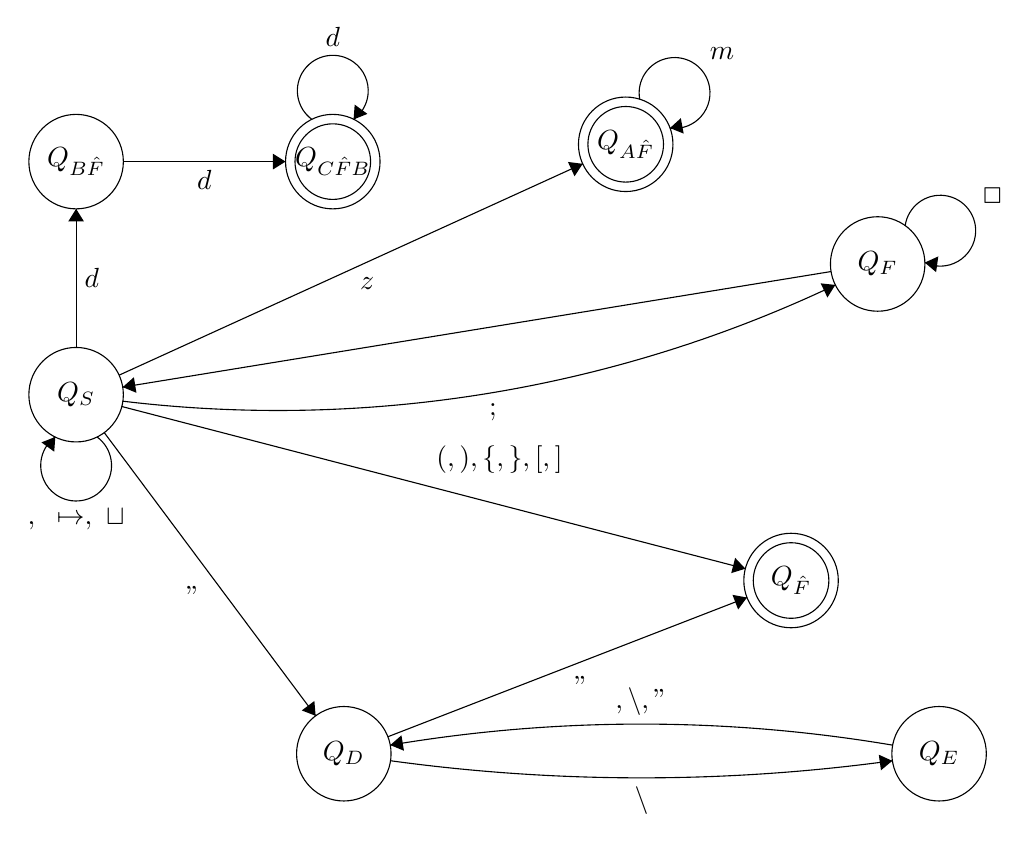
\begin{tikzpicture}[scale=0.2]
\tikzstyle{every node}+=[inner sep=0pt]
\draw [black] (11.9,-24.9) circle (3);
\draw (11.9,-24.9) node {$Q_{S}$};
\draw [black] (11.9,-10.1) circle (3);
\draw (11.9,-10.1) node {$Q_{B\hat{F}}$};
\draw [black] (46.8,-9) circle (3);
\draw (46.8,-9) node {$Q_{A\hat{F}}$};
\draw [black] (46.8,-9) circle (2.4);
\draw [black] (57.3,-36.7) circle (3);
\draw (57.3,-36.7) node {$Q_{\hat{F}}$};
\draw [black] (57.3,-36.7) circle (2.4);
\draw [black] (28.2,-10.1) circle (3);
\draw (28.2,-10.1) node {$Q_{C\hat{F}B}$};
\draw [black] (28.2,-10.1) circle (2.4);
\draw [black] (28.9,-47.7) circle (3);
\draw (28.9,-47.7) node {$Q_{D}$};
\draw [black] (62.8,-16.6) circle (3);
\draw (62.8,-16.6) node {$Q_{F}$};
\draw [black] (66.7,-47.7) circle (3);
\draw (66.7,-47.7) node {$Q_{E}$};
\draw [black] (11.9,-21.9) -- (11.9,-13.1);
\fill [black] (11.9,-13.1) -- (11.4,-13.9) -- (12.4,-13.9);
\draw (12.4,-17.5) node [right] {$d$};
\draw [black] (14.63,-23.66) -- (44.07,-10.24);
\fill [black] (44.07,-10.24) -- (43.13,-10.12) -- (43.55,-11.03);
\draw (30.38,-17.46) node [below] {$z$};
\draw [black] (14.8,-25.65) -- (54.4,-35.95);
\fill [black] (54.4,-35.95) -- (53.75,-35.26) -- (53.5,-36.23);
\draw (38.78,-29.93) node [above] {$(,),\{,\},[,]$};
\draw [black] (47.69,-6.147) arc (190.39718:-97.60282:2.25);
\draw (52.92,-3.63) node [above] {$m$};
\fill [black] (49.61,-7.97) -- (50.48,-8.32) -- (50.3,-7.34);
\draw [black] (14.9,-10.1) -- (25.2,-10.1);
\fill [black] (25.2,-10.1) -- (24.4,-9.6) -- (24.4,-10.6);
\draw (20.05,-10.6) node [below] {$d$};
\draw [black] (26.877,-7.42) arc (234:-54:2.25);
\draw (28.2,-2.85) node [above] {$d$};
\fill [black] (29.52,-7.42) -- (30.4,-7.07) -- (29.59,-6.48);
\draw [black] (13.69,-27.31) -- (27.11,-45.29);
\fill [black] (27.11,-45.29) -- (27.03,-44.35) -- (26.23,-44.95);
\draw (19.82,-37.69) node [left] {$"$};
\draw [black] (60.113,-17.935) arc (-64.62048:-96.8567:82.559);
\fill [black] (60.11,-17.93) -- (59.18,-17.83) -- (59.61,-18.73);
\draw (38.37,-25.41) node [below] {$;$};
\draw [black] (63.733,-48.145) arc (-82.19306:-97.80694:117.299);
\fill [black] (63.73,-48.15) -- (62.87,-47.76) -- (63.01,-48.75);
\draw (47.8,-49.73) node [below] {$\backslash$};
\draw [black] (31.7,-46.62) -- (54.5,-37.78);
\fill [black] (54.5,-37.78) -- (53.58,-37.61) -- (53.94,-38.54);
\draw (44,-42.72) node [below] {$"$};
\draw [black] (31.85,-47.154) arc (99.59557:80.40443:95.687);
\fill [black] (31.85,-47.15) -- (32.72,-47.51) -- (32.56,-46.53);
\draw (47.8,-45.31) node [above] {$\blacksquare,\backslash,"$};
\draw [black] (64.545,-14.174) arc (172.01431:-115.98569:2.25);
\draw (69.44,-12.27) node [right] {$\Square$};
\fill [black] (65.79,-16.51) -- (66.51,-17.12) -- (66.65,-16.12);
\draw [black] (13.223,-27.58) arc (54:-234:2.25);
\draw (11.9,-32.15) node [below] {$\dlsh,\mbox{ }\mapsto,\mbox{ }\sqcup$};
\fill [black] (10.58,-27.58) -- (9.7,-27.93) -- (10.51,-28.52);
\draw [black] (59.84,-17.08) -- (14.86,-24.42);
\fill [black] (14.86,-24.42) -- (15.73,-24.78) -- (15.57,-23.79);
\draw (36.1,-19.97) node [above] {$\dlsh$};
\end{tikzpicture}
\end{center}


\end{document}
